\mysubsection{Suivi du calendrier du projet}\label{Suivi}

En raison des problèmes dans le déroulement de nos activités soit de performance du système, soit de manque de temps, on n'a pas suivi parfaitement le calandrier initiale du projet. On a essayé de l'adapter pour accomplir le plus grand nombre possible de tâches. Dans la table suivante, on a la vraie distribution temporelle de nos activités.

\begin{figure}[H]
	\begin{center}	
		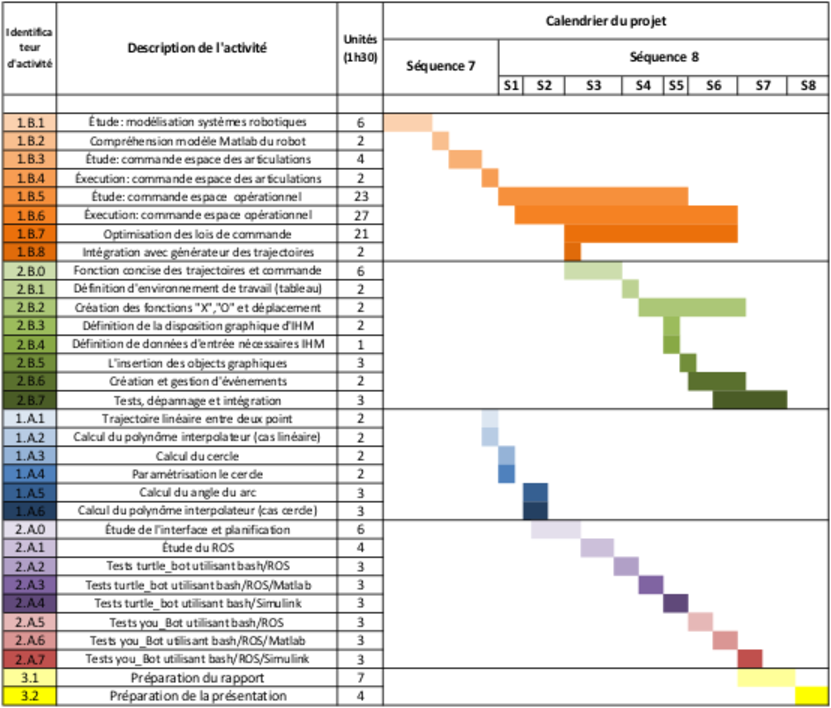
\includegraphics[width=\textwidth]{./Cronograma2}
		\caption{Calendrier de suivi du projet.}
		\label{fig:cronograma2}
	\end{center}
\end{figure}

À propos de la commande, on a beaucoup changé le calandrier original parce qu'on a resté longtemps en train d'essayer plusieurs types différents de contrôleurs jusqu'à avoir un avec des performances satisfaisantes.